\documentclass[main.tex]{subfiles} % Subfile-Class

%==============================================================================%
%                                   Subfile                                    %
%==============================================================================%

\begin{document}

% Template

\section{Parametrierung HcSr04 Ultraschallsensor}~\label{apdx:FilterDimensionierungHcSr04}

Dieser Abschnitt behandelt Die Parametrierung des HcSr04. Dabei handelt es sich
um einen sehr kostengünstigen Ultraschallsensor, welcher über das Echo eines
selbst ausgestossenen Ultraschall-Bursts auf die gemessene Distanz
rückschliessen lässt.

\subsection*{Ansteuerung}

Das Datenblatt dieses Sensor schreibt folgenden Steuerablauf vor:

\begin{enumerate}
    \item Fallende Flanke am Triggereingang für mindestens $10 \mu s$
    \item Modul sendet 40kHz Burst für die dauer von $200 \mu s$
    \item Kommt Echo zurück, fällt der Echo Ausgang auf Low
    \item nach ca. $20 ms$ kann eine erneute Messung stattfinden.
\end{enumerate}

In der Firmware des MotionControllers wird dies durch einen eigenen Sensor-Task
gelöst, der nach dem Auslösen eines Triggers blockiert wird. Kommt das Echo
zurück, wird ein Interrupt ausgelöst, der die Umrechnung der Zeitdifferenz in
eine Entfernung über die Schallgeschwindigkeit auslöst. Ist dies geschehen,
folgen weitere Berechnungen wie z.B. eine zeitdiskrete Tiefpassfilterung. Am
Ende des Messzyklus geht die Task in den Ruhezustand, bis nach ~50 ms eine neue
Messung durchgeführt wird.

Diese Zeitdifferenz wurde gewählt, um zu verhindern, dass der Echo-Pin ein Echo
aus einem früheren Messzyklus anzeigt.

\subsection*{Sensorverhalten}
Die Genauigkeit dieses Sensors ist nach einem Datenblatt mit +-3mm angegeben.

\begin{figure}[H]
    \centering
    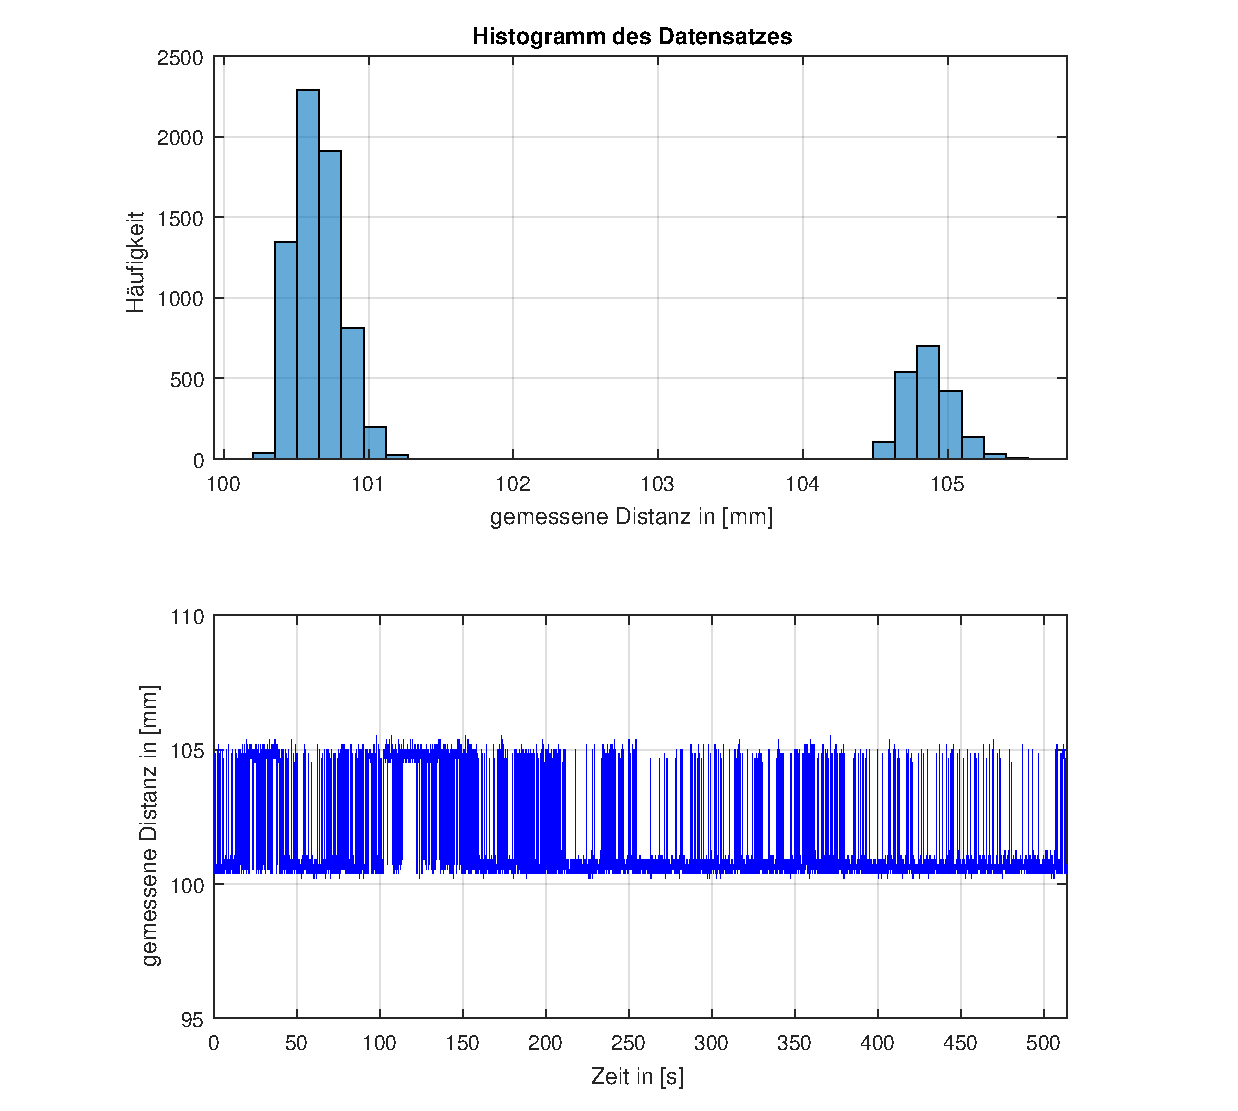
\includegraphics[width=0.75\linewidth]{./fig_Parametrierung_HcSr04/Messverteilung_HcSr04.pdf}
    \caption{Histogramm Sensorauswertung}~\label{fig:HistogrammHcSr04}
\end{figure}

Abbildung~\ref{fig:HistogrammHcSr04} zeigt die Auswertung eines Datensatzes von
fast 9000 Messungen, die mit dem Roboter aufgenommen wurden. Dabei ist ein
Hindernis in $\approx 100mm$ Entfernung gemessen.

Die Auswertung zeigt, dass die Verteilung der Messwerte grundsätzlich einer
Normalverteilung folgt. Die vom Hersteller angegebene Abweichung von +-3 mm
beschreibt jedoch keine Standardabweichung aus einer Gaussverteilung, sondern
vielmehr sprunghafte Veränderungen, die sich im Histogramm in der zweiten,
kleineren Gaussglocke bei einer Distanz von $\approx 105mm$ zeigen.

Etwa $20 \%$ aller Messungen liegen in dieser zweiten Glocke, was als eher
kritisch anzusehen ist. Um das Fahrzeug abzubremsen, wird die Annäherung eines
Hindernisses in \textit{Bremsdistanz} abgewartet. Da der Roboter mit einer
Geschwindigkeit von $0.5 \frac{m}{s}$ fährt, bewegt er sich zwischen jedem
Messzyklus um $30 mm$. Tritt nun einer der $20\%$-Ausreisser genau in dem
Moment auf, in dem das Fahrzeug eigentlich bremsen sollte, oder wird ein Wert
auch nur $1mm$ weiter weg gemessen, als das Fahrezg beginnen würde zu bremsen,
so wird das \textit{Bremsmoment} erst einen Messzyklus später erkannt, was zu
einem Verfehlen des Hindernisses um $\approx. 30 mm$ führt. Da diese Messfehler
mit einer Wahrscheinlichkeit von $1:5$ auftreten, besteht hier dringender
Handlungsbedarf.

\subsection*{Tiefpassfilterung}

\subsubsection*{Einfacher IIR-Ansastz}

Um die Ausreisser in den Gruff zu bekommen, wird ein Tiefpassfilter eingesetzt.
Eine einfache zeitdiskrete rekursive Tiefpassfilterung erster Ordnung hat die
Form

\[
    y[k] = (1 - \alpha) x[k] + \alpha y[k - 1]
\]

Wobei $x[k]$ den Messwert zum aktuellen Zeitpunkt und $y[k]$ den Filterausgang
kennzeichnet.

Dieser Filter könnte mit einem konservativ gewählten Faktor $\alpha$ die
entsprechenden Sprünge und das Rauschen bereits stark unterdrücken. Die Folge
ist jedoch, wie bereits aus der Filtergleichung ersichtlich, dass die Messwerte
stark verzögert werden.

\begin{figure}[H]
    \centering
    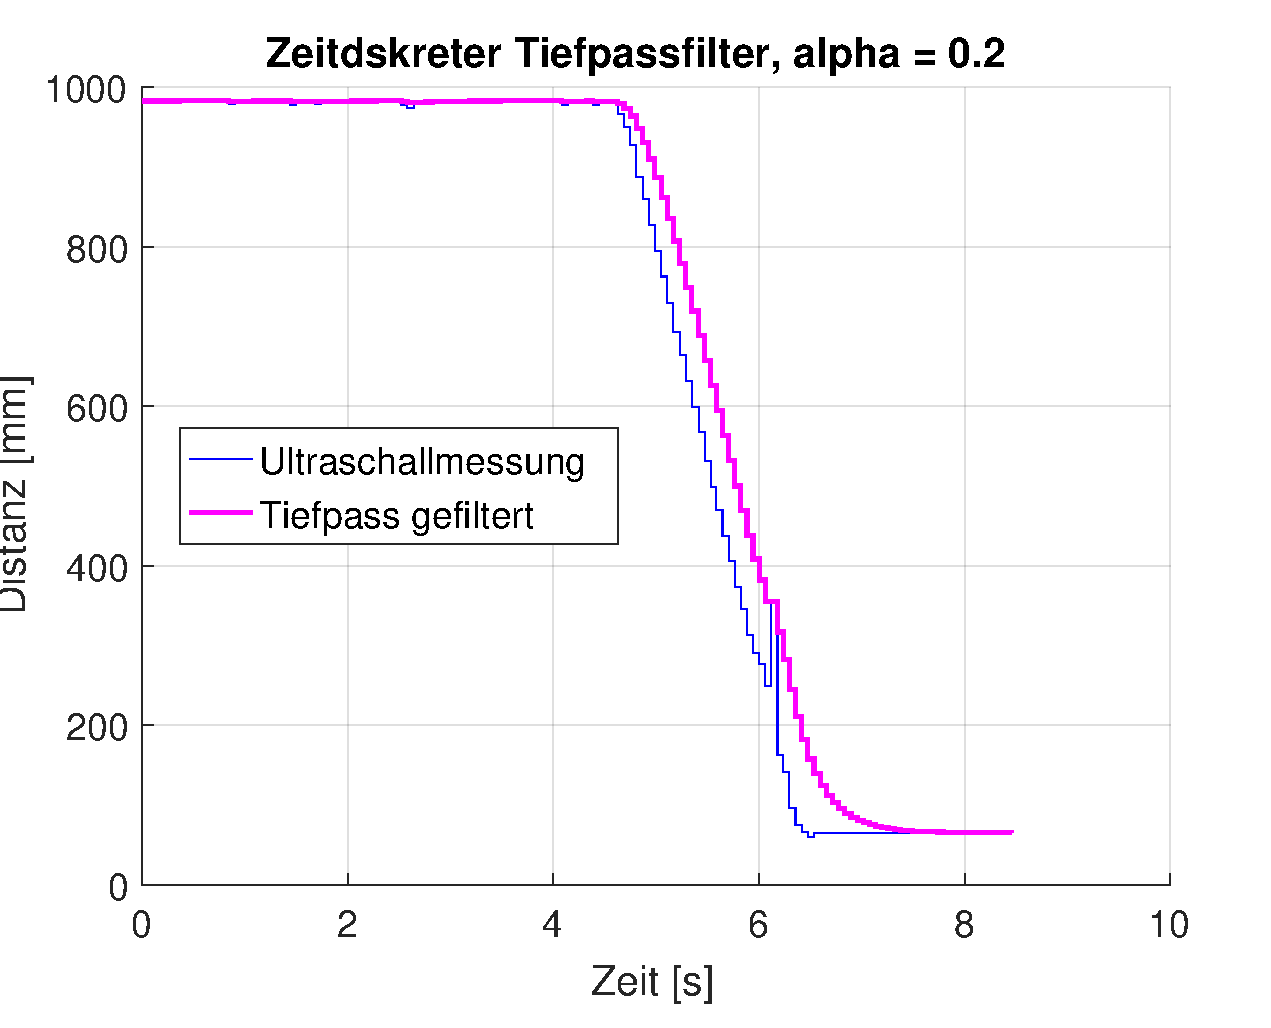
\includegraphics[width=0.5\linewidth]{./fig_Parametrierung_HcSr04/Einfacher_Tiefpass_HcSr04.pdf}
    \caption{Tiefpass angewendet auf Annäherungsfahrt}~\label{fig:EinfacherTiefpassHcSr04}
\end{figure}

Abbildung~\ref{fig:EinfacherTiefpassHcSr04} zeigt die Anwendung eines
Tiefpasses auf eine Messreihe des realen Roboters. Dabei werden die Sensorwerte
während einer Fahrt auf ein Hinternis ausgewertet.

Der Koeffizient $\alpha = 0.2$ wurde so gewählt, dass der Messwertsprung bei
knapp über $6s$ noch einigermassen herausgefiltert wird. Diese Abbildung zeigt
auch, wie schnell es passieren kann, dass der Sensorwert in dem Moment, in dem
gebremst werden soll, plötzlich zu springen beginnt.

Ein grosser Nachteil dieses Ansatzes ist ist die starke Zeitverzögerung der
Messwerte, wodurch der richtige Abstand, bei dem der Roboter rechtzeitig
bremsen sollte, nicht erreicht wird.

\subsubsection*{Verbesserung durch Modellierung der Fahrzeugposition}~\label{apdx:Adaptiver_Tiefpass}

Der Tiefpassfilter filtert schnelle Änderungen des Messwerts heraus. Das System
hat jedoch eine bekannte Änderung: die Annäherung an ein Hindernis mit der
Geschwindigkeit $v[k]$. Mit dieser Geschwindigkeit kann die Änderung der
Hindernisposition vorhergesagt werden. Wird nun der Wert $y[k - 1]$ bereits um
diese bekannte Änderung interpoliert, kann das Tiefpassfilter bereits deutlich
\textit{beschleunigt} werden, da durch die Vorhersage immer ein aktueller Wert
zur Verfügung steht.

Diese Interpolation zwischen den Messwerten mit der bekannten Geschwindigkeit
erlaubt es ausserdem, diese Vorhersage häufiger abzufragen, als der Sensor sie
erfasst. Dadurch erhöht sich rechnerisch die Auflösung der Werte zwischen den
Messzyklen.

Die \textit{Vorhersage} wird wie folgt beschrieben:
\[
    y_{pred}[k] = y[k - 1] + v[k] \cdot dt
\]

Jedes Mal, wenn ein neuer Messwert zur Verfügung steht, kann der Tiefpassfilter
aus dem vergangenen Abschnitt darauf angesetzt werden. Was sich nun allerdings
ändert, ist, dass $y[k - 1]$ durch die Vorhersage $y_{pred}[k]$ ersetzt wird.
Dadruch wird die die Zeitverzögerung des Tiefpasses bereits massiv verringert.
Der Tiefpassfilter hat so eine gewisse Korrekturfunktion für die vorrausgesagte
Distanz.

Die \textit{Korrektur} dieser Vorhersage lässt sich wie folgt beschreiben:
\[
    y[k] = (1 - \alpha) x[k] + \alpha y_{pred}[k]
\]

\begin{figure}[H]
    \centering
    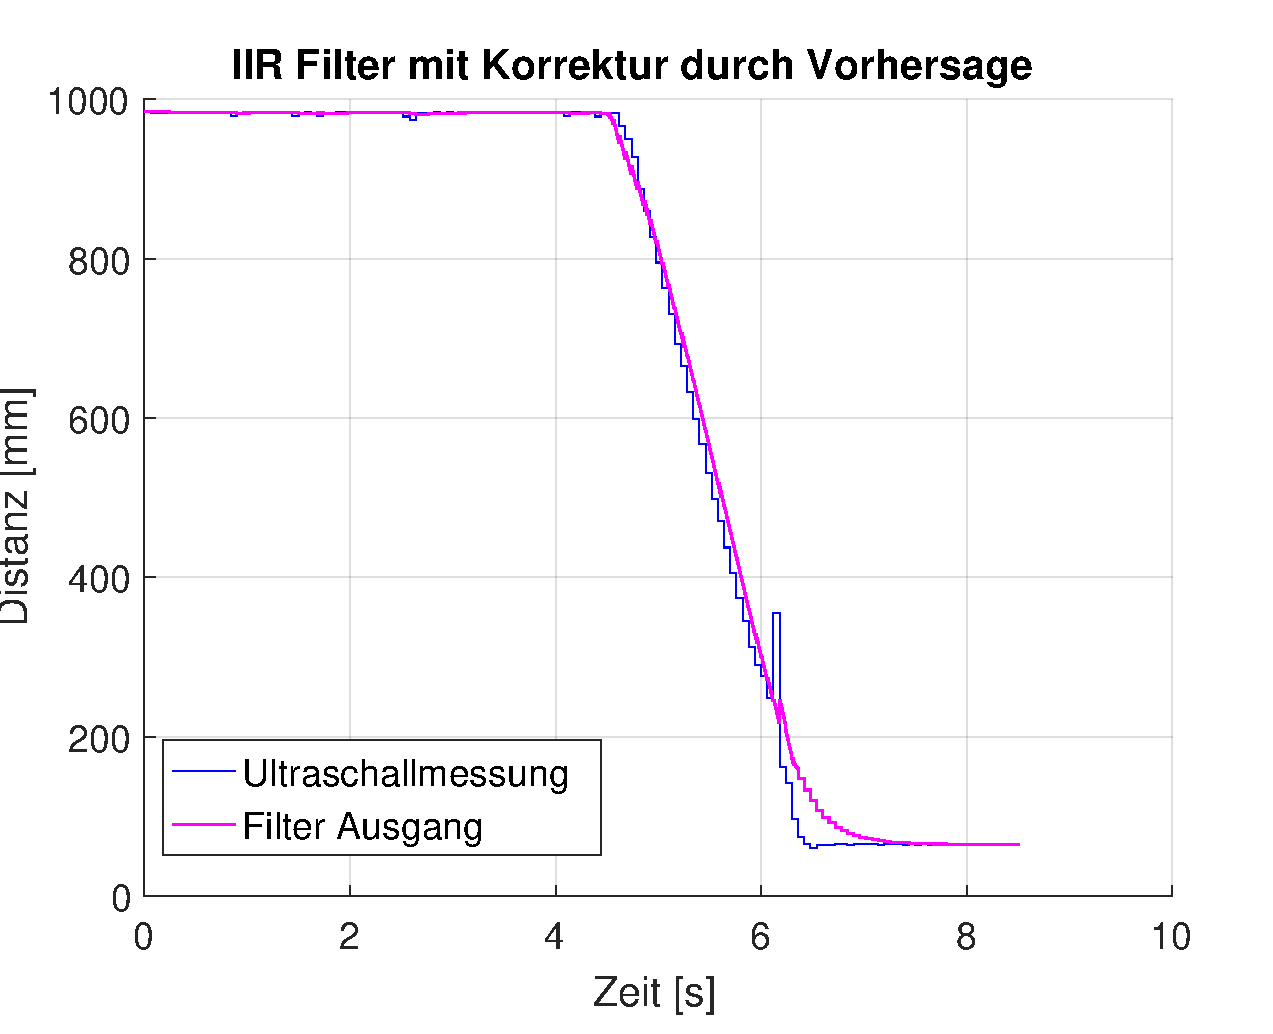
\includegraphics[width=0.5\linewidth]{./fig_Parametrierung_HcSr04/Einfacher_Tiefpass_HcSr04_Erweitert_durch_Modell.pdf}
    \caption{Erweiterter Tiefpass angewendet auf Annäherungsfahrt}~\label{fig:EinfacherTiefpassHcSr04_Erweitert}
\end{figure}

Abbildung~\ref{fig:EinfacherTiefpassHcSr04_Erweitert} zeigt die Wirkung dieses
erweiterten Tiefpassfilters. Die Geschwindigkeit, mit der die Messwerte zur
Verfügung stehen, hat sich bereits massiv verbessert. Nun kann die
Geschwindigkeit nicht besser bestimmt werden, als sie binär zwischen
\texttt{Vmax} und \texttt{Vmin} zu betrachten. Ausserdem ist die
Geschwindigkeit nur ein theoretischer Wert, der im Voraus berechnet wird.
Geschwindigkeitsschwankungen durch Lenkbewegungen, ungenaue Radabmessungen oder
Rundungsfehler der MCU führen zu Abweichungen in der Vorhersage. In
Abbildung~\ref{fig:EinfacherTiefpassHcSr04_Erweitert} ist dies auch an einer
gewissen Drift zu späteren Messwerten erkennbar. Eine gewisse
\textit{Korrektur} der Geschwindigkeitsvorhersage wäre daher wünschenswert.

\subsubsection*{Verbesserung durch Geschwindigkeitskorrektur}

Bei jeder Messung wird der Ausgangswert des Filters durch den Tiefpass in eine
bestimmte Richtung korrigiert. Die anschliessende Positionsvorhersage basiert
jedoch wieder auf falschen Werten. Wünschenswert wäre daher eine dynamische
Anpassung/Korrektur der Schätzung in Abhängigkeit davon, wie gut der zuletzt
gemessene Wert mit dem erwarteten Wert übereinstimmt.

Dazu wird nun die zusätzliche Konstante $c_v$ eingeführt:

\[
    \Delta x[k] = x[k] - y_{pred}[k]
\]
\[
    c_v[k] = \frac{\Delta x[k]}{\Delta x[k] + \beta}
\]

Der Faktor $c_v[k]$ repräsentiert damit einen auf 1 normierten Wert,
\textit{wie gut} die letzte Schätzung gewesen ist. Über die Konstante $\beta$
lässt sich einstellen, wie stark $c_v[k]$ auf eine Schätzabweichung reagiert.

Mit dieser Information lässt sich nun für die nachfolgende Schätz-Phase die
Geschwindigkeit mit welcher gerechet wird, korrigieren.

Die \textit{Vorhersage} wird nun wie folgt beschrieben:
\[
    y_{pred}[k] = y[k - 1] + (c_v[k] \cdot v[k]) \cdot dt
\]
Wohingegen die Korrekturphase unverändert bleibt.

Durch diese Massnahme kann die Filterausgabe nochmals verbessert werden, da die
Positionsschätzung nun entsprechend der Messabweichung korrigiert wird. Damit
diese Korrektur funktioniert, ist eine Messabweichung erforderlich. Dadurch
pendelt die Schätzung $y_{pred}[k]$ immer um den aktuellen Messwert $x[k]$. Um
die Geschwindigkeitskorrektur auch bei nachfolgenden Schätzungen in den Griff
zu bekommen und die Schätzung korrekt an den nächsten Messwert anzunähern, wird
zusätzlich ein minimaler Integrator hinzugefügt, der die letzten
Messabweichungen aufintegriert und bei der nächsten Schätzung berücksichtigt.
Dadurch wird das System träger, was aber für ein Tiefpassverhalten erwünscht
ist. Dieser Integrator soll während der Messung ebenfalls Korrekturen erfahren
können. Deshalb wird noch der Korrekturfaktor $c_i$ eingeführt, der wie $c_v$
nur mit dem Parameter $\gamma$ bestimmt wird:

\[
    c_i[k] = \frac{\Delta x[k]}{\Delta x[k] + \gamma}
\]

Final wird die Vorhersage nun also wie folgt beschrieben:
\[
    y_{pred}[k] = y[k - 1] + (c_v[k] \cdot v[k]) \cdot dt + (c_i[k] \cdot k_i) \cdot \int \Delta x[k]\,dk
\]

\begin{figure}[H]
    \centering
    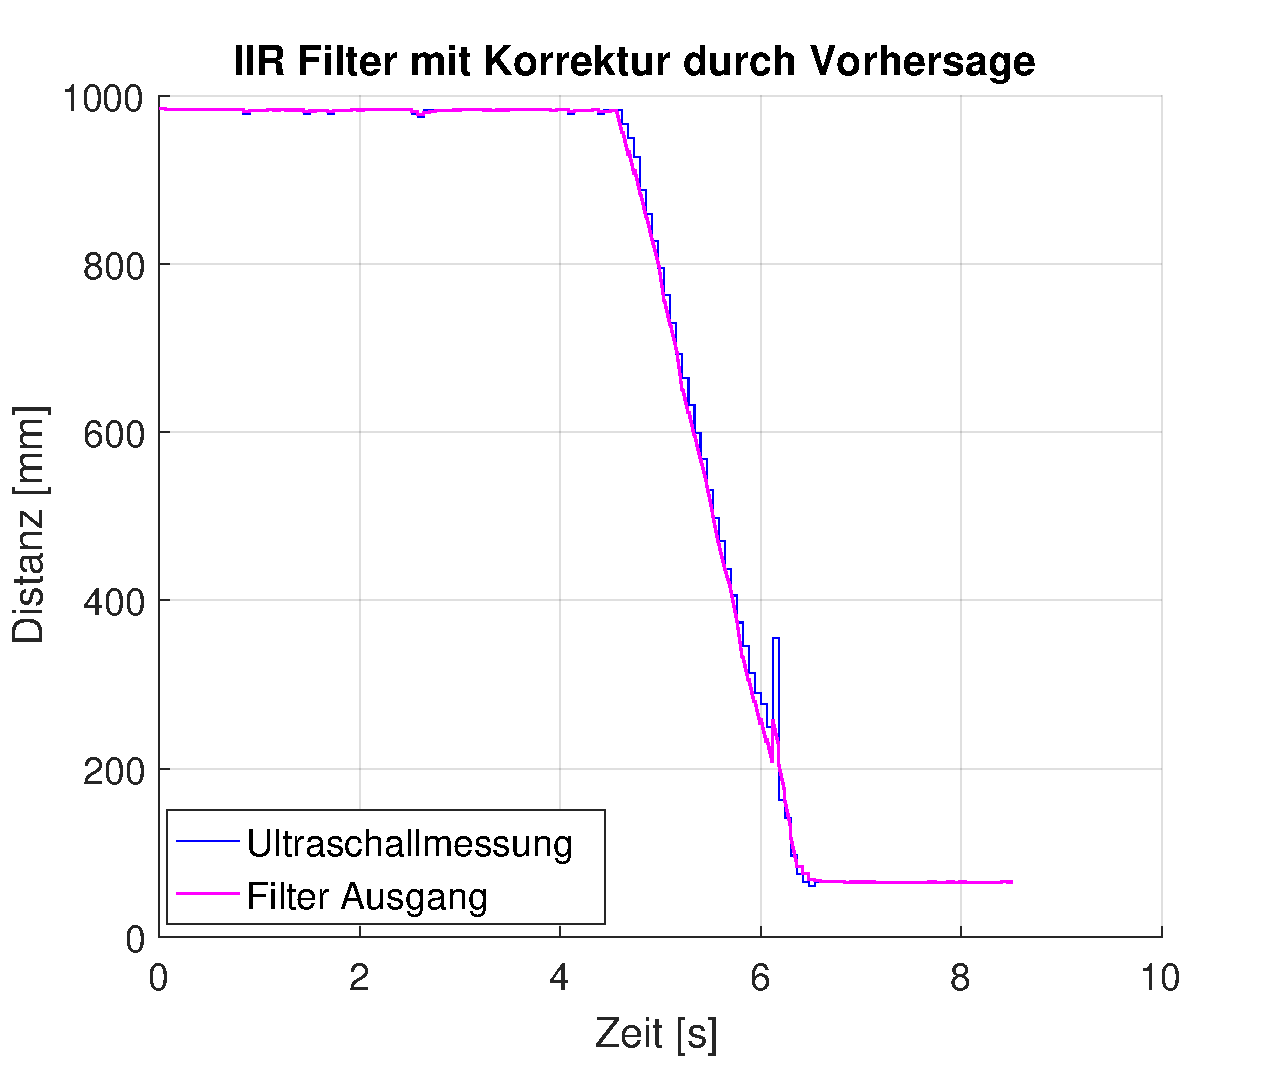
\includegraphics[width=0.5\linewidth]{./fig_Parametrierung_HcSr04/Einfacher_Tiefpass_HcSr04_V_Korrigiert.pdf}
    \caption{Finaler Filter angewendet auf Annäherungsfahrt}~\label{fig:EinfacherTiefpassHcSr04_V_Korrigiert}
\end{figure}

Abbildung~\ref{fig:EinfacherTiefpassHcSr04_V_Korrigiert} zeigt die Anwendung
des ermittelten Filters auf die aufgezeichnete Messreihe. Der Peak kurz vor dem
Abbremszeitpunkt konnte nicht vollständig eliminiert werden, jedoch ist es
nicht möglich, die sporadischen Peaks ohne grosse Einbussen in der Dynamik zu
unterdrücken.

Um auch mit diesen sporadischen Peaks umgehen zu können, wird der Roboter nun
mit einem kleinen Sicherheitsabstand vor dem Hindernis positioniert. Die letzte
Strecke zur Greifposition wird erst zurückgelegt, nachdem der Median aus einer
gewissen Reihe von Messungen ermittelt wurde.

\end{document}

